\chapter[Obtaining FDTD Spectral Information]{Obtaining Spectral
Information from an FDTD Simulation \label{chap:spectrum}}

%\setcounter{page}{1}
\renewcommand{\thefootnote}{\fnsymbol{footnote}}
\footnotetext[2]{Lecture notes by John Schneider.  {\tt
fdtd-spectral.tex}}

\section{Introduction}

The majority of instructional material concerning electromagnetics is
expressed in terms of harmonic, or frequency-domain, signals.  A
temporal dependence of $\exp(j\omega t)$ is understood and therefore
one only has to consider the spatial variation.  In the frequency
domain, the fields and quantities such as the propagation constant and
the characteristic impedance are represented by complex numbers.
These complex numbers give the magnitude and phase of the value and
will be functions of frequency.  In this chapter a caret (hat) will be
used to indicate a complex quantity and one should keep in mind that
complex numbers are inherently tied to the frequency domain.  Given
the frequency-domain representation of the field at a point, the
temporal signal is recovered by multiplying by $\exp(j\omega t)$ and
taking the real part.  Thus a 1D harmonic field propagating in the
$+x$ direction could be written in any of these equivalent forms
\begin{equation}
E_z(x,t) = 
  \Re\!\left[\hE_z^+(x,t)\right]
   = 
  \Re\!\left[\hE_z^+(x)e^{j\omega t}\right]
   = 
  \Re\!\left[\hE_a^+e^{-\hgamma x}e^{j\omega t}\right]
   = 
  \Re\!\left[\hE_a^+e^{-(\alpha+j\beta) x}e^{j\omega t}\right],
\end{equation}
where $\Re[]$ indicates the real part.  $\hE_z^+(x)$ is the
frequency-domain representation of the field (i.e., a phasor that is a
function of position), $\hgamma$ is the propagation constant which has
a real part $\alpha$ and an imaginary part $\beta$, and $\hE_a^+$ is a
complex constant that gives the amplitude of the wave (it is
independent of position; the superscript ``$+$'' is merely used to
emphasize that we are discussing a wave propagating in the $+x$
direction).  Note that if more than a single frequency is present,
$\hE_a^+$ does not need to be the same for each frequency.

More generally, $\hE_a^+$ will be a function of frequency (we could
write this expressly as $\hE_a^+(\omega)$ but the caret implicitly
indicates dependence on frequency).  To construct a temporal that
consists of a multiple frequencies, or even a continuous spectrum of
frequencies, one must sum the contributions from each frequency such
as is done with a Fourier integral.

In FDTD simulations the time-domain form of the signal is obtained
directly.  However, one often is interested in the behavior of the
fields as a function of frequency.  As has been discussed in Sec.\
\ref{sec:fftMapping}, one merely has to take the Fourier transform of
a signal to obtain its spectral content.  This transform, by itself,
is typically of little use.  One has to normalize the signal in some
way.  Knowing what came out of a system is rather meaningless unless
one knows what went into the system.  Here we will work through a
couple of simple examples to illustrate how a broad range of spectral
information can be obtained from FDTD simulations.

\section[Transmission through Planar Interface]{Transmission through a
Planar Interface (Continuous World) \label{sec:contTrans}}

Consider the planar interface at $x=0$ between two media as
depicted in Fig.\ \ref{fig:planarInterface}.  We restrict
consideration to electric polarization in the $z$ direction and assume
the incident field originates in the first medium.
\begin{figure}
  \begin{center}
  \vspace{1.5in} %%%%%%%%%%%%%% REMOVE ME!!!!!!!
 %  \epsfig{width=5.in,file=Code/C4/max-elec-field.eps}
  \end{center}
  \caption{Planar interface between two media.  The interface is at
 $x=0$ and a wave is incident on the interface from the left.  When the
 impedances of the two media are not matched, a reflected wave must
 exist in order to satisfy the boundary conditions.}
  \label{fig:planarInterface}
\end{figure}
In the frequency domain, the incident, reflected, and transmitted
fields are given by
\begin{eqnarray}
  \hE_z^i(x) \!&=&\! \hE_{a1}^+ e^{-\hgamma_1 x} 
    \qquad \mbox{\hspace{.92in}incident},\\
  \hE_z^r(x) \!&=&\! \hE_{a1}^- e^{+\hgamma_1 x} =
                   \hG \hE_{a1}^+ e^{+\hgamma_1 z} \qquad \mbox{reflected},\\
  \hE_z^t(x) \!&=&\! \hE_{a2}^+ e^{-\hgamma_2 x} =
                   \hT \hE_{a1}^+ e^{-\hgamma_2 x} \qquad \mbox{transmitted},
\end{eqnarray}
where $\hG$ is the reflection coefficient, $\hT$ is the transmission
coefficient, and $\hgamma_n$ is the propagation constant given by
$j\omega\sqrt{\mu_n(1-j\sigma^m_n/\omega\mu_n)
  \epsilon_n(1-j\sigma_n/\omega\epsilon_n)}$ where the $n$ indicates
the medium and $\sigma^m$ is the magnetic conductivity.  The amplitude
of the incident field $\hE_{a1}^+$ is, in general, complex and a
function of frequency.  By definition $\hG$ and $\hT$ are
\begin{eqnarray}
  \hG &=& \left.\frac{\hE_z^r(x)}{\hE_z^i(x)}\right|_{x=0} =
              \frac{\hE_{a1}^-}{\hE_{a1}^+}, \\
       \hT &=& \left.\frac{\hE_z^t(x)}{\hE_z^i(x)}\right|_{x=0} = 
              \frac{\hE_{a2}^+}{\hE_{a1}^+}.
\end{eqnarray}
The fact that these are defined at $x=0$ is important.

The magnetic field is related to the electric field by
\begin{eqnarray}
  \hH_y^i(x) &=& -\frac{1}{\heta_1}\hE_z^i(x), \\ 
  \hH_y^r(x) &=& \frac{1}{\heta_1}\hE_z^r(x), \\ 
  \hH_y^t(x) &=& -\frac{1}{\heta_2}\hE_z^t(x),
\end{eqnarray}
where the characteristic impedance $\heta_n$ is given by
$\sqrt{\mu_n(1-j\sigma^m_n/\omega\mu_n)/
  \epsilon_n(1-j\sigma_n/\omega\epsilon_n)}$.  Since the magnetic and
electric fields are purely tangential to the planar interface, the sum
of the incident and reflected field at $x=0$ must equal the
transmitted field at the same point.  Matching the boundary condition
on the electric field yields
\begin{equation}
  1 + \hG = \hT,
  \label{eq:matchingFields}
\end{equation}
while matching the boundary conditions on the magnetic field produces
\begin{equation}
 \frac{1}{\heta_1}(1 - \hG) = \frac{1}{\heta_2}\hT.
\end{equation}
Solving these for $\hT$ yields
\begin{equation}
  \hT = \frac{2\heta_2}{\heta_1+\heta_2}.
  \label{eq:transCoefSpectral}
\end{equation}
Using this in \refeq{eq:matchingFields} the reflection coefficient is
found to be
\begin{equation}
  \hG = \frac{\heta_2-\heta_1}{\heta_2+\heta_1}.
  \label{eq:refCoefSpectral}
\end{equation}

\section{Measuring the Transmission Coefficient Using FDTD
\label{sec:measureTrans}}

Now consider two FDTD simulations.  The first simulation will be used
to record the incident field.  In this simulation the computational
domain is homogeneous and the material properties correspond to that
of the first medium.  The field is recorded at some observation point
$x_1$.  Since nothing is present to interfere with the incident field,
the recorded field will be simply the incident field at this location,
i.e, $E_z^i(x_1,t)$.  In the second simulation the second medium is
present, i.e., the space is no longer homogeneous.  We record the
fields at the same observation point but we ensure the point was
chosen such that it is located in the second medium (i.e., the
interface is to the left of the observation point).  Performing an
FDTD simulation in this case yields the transmitted field
$E_z^t(x_1,t)$.  The goal now is to obtain the transmission
coefficient using the temporal recordings of the field obtained from
these two simulations.

{\em Note} that in this section we will not distinguish between the
way in which field propagate in the continuous world and the way in
which they propagate in the FDTD grid.  In
Chap.\ \ref{chap:dispersion} we will discuss in some detail how these
differ.

One cannot use $E_z^t(x_1,t)/E_z^i(x_1,t)$ to obtain the transmission
coefficient.  The transmission coefficient is inherently a
frequency-domain concept and currently we have time-domain signals.
The division of these temporal signals is essentially meaningless
(e.g., the result is undefined when the incident signal is zero).

The incident and transmitted fields must be converted to the frequency
domain using a Fourier transform.  Thus one obtains
\begin{eqnarray}
 \hE_z^i(x_1) &=& {\cal F}\left(E_z^i(x_1,t)\right), \\
 \hE_z^t(x_1) &=&  {\cal F}\left(E_z^t(x_1,t)\right),
\end{eqnarray} 
where ${\cal F}$ indicates the Fourier transform.  The division of
these two functions {\em is} meaningful---at least at all frequencies
where $\hE_z^i(x_1)$ is non-zero.  (At frequencies where
$\hE_z^i(x_1)$ is zero, there is no incident spectral energy and hence
one cannot obtain the transmitted field at those particular
frequencies.  In practice it is relatively easy to introduce energy
into an FDTD grid that spans a broad range of frequencies.)

Since the observation point was not specified to be on the boundary,
the ratio of these field fields is
\begin{equation}
  \frac{\hE_z^t(x_1)}{\hE_z^i(x_1)} =
  \frac{\hE_{a2}^+e^{-\hgamma_2 x_1}}{\hE_{a1}^+e^{-\hgamma_1 x_1}} =
  \frac{\hE_{a2}^+}{\hE_{a1}^+}e^{(\hgamma_1-\hgamma_2) x_1} =
  \hT e^{(\hgamma_1-\hgamma_2) x_1}.
\end{equation}
Solving this for $\hT$ yields
\begin{equation}
  \hT(\omega) = e^{(\hgamma_2-\hgamma_1) x_1}
  \frac{\hE_z^t(x_1)}{\hE_z^i(x_1)}.
  \label{eq:transCoefShifted}
\end{equation}

To demonstrate how the transmission coefficient can be
reconstructed from FDTD simulations, let us consider an example where
the first medium is free space and the second one has a relative
permittivity $\epsilon_r$ of $9$.  In this case
$\hgamma_1=j\omega\sqrt{\mu_0\epsilon_0}=j\beta_0$ and
$\hgamma_2=j\omega\sqrt{\mu_0 9\epsilon_0}=j3\beta_0$.
Therefore \refeq{eq:transCoefShifted} becomes
\begin{equation}
  \hT(\omega) = e^{j(3\beta_0-\beta_0) x_1}
  \frac{\hE_z^t(x_1)}{\hE_z^i(x_1)}
  = e^{j2\beta_0 x_1}
  \frac{\hE_z^t(x_1)}{\hE_z^i(x_1)}.
\end{equation}
The terms in the exponent can be written
\begin{equation}
  2\beta_0 x_1 = 2\frac{2\pi}{\lambda}x_1 = 
  \frac{4\pi}{\ppw\Delx}N_1\Delx =
  \frac{4\pi}{\ppw}N_1
  \label{eq:transExponent}
\end{equation}
where $N_1$ is the number of spatial steps between the interface and
the observation point at $x_1$ and, as was discussed in Chap.\
\ref{chap:dimensionless}, $\ppw$ is the number of spatial steps per a
free-space wavelength of $\lambda$.

The continuous-world transmission coefficient can be calculated quite
easily from \refeq{eq:transCoefSpectral} and this provides a reference
solution.  Ideally the FDTD simulation would yield this same value for
all frequencies.  For this particular example the characteristic
impedance of the first medium is $\heta_1=\eta_0$ while for the second
medium it is $\heta_2=\eta_0/3$.  Thus the transmission coefficients
is
\begin{equation}
  \hT_{\mbox{\scriptsize exact}} = \frac{2\eta_0/3}{\eta_0+\eta_0/3} = 1/2.
  \label{eq:transExact}
\end{equation}
Note that this is a real number and independent of frequency (so the
tilde on $T$ is somewhat misleading).

For the FDTD simulations, let us record the field 80 spatial steps
away from the interface, i.e., $N_1=80$, and run the simulation for
8192 time steps, i.e., $N_T=8192$.  The simulation is run at the
Courant limit $S_c=1$.  The source is a Ricker wavelet discretized so
that the peak spectral content exists at 50 points per wavelength
($N_P=50$).  From Sec.\
\ref{sec:fftMapping}, recall the relationship between the points per
wavelength $\ppw$ and frequency index $N_{\mathrm{freq}}$ which is
repeated below:
\begin{equation}
  N_{\mathrm{freq}} = \frac{N_T}{\ppw} S_c.
\end{equation}
With a Courant number of unity and 8192 time steps, the points per
wavelength for any given frequency (or spectral index) is given by
\begin{equation}
  \ppw = \frac{8192}{N_{\mathrm{freq}}}.
\end{equation}
Combining this with \refeq{eq:transCoefShifted} and
\refeq{eq:transExponent} yields
\begin{equation}
  \hT_{\mbox{\scriptsize FDTD}}
  = e^{j\left(\frac{4\pi N_1N_{\mathrm{freq}}}{8192}\right)}
  \frac{\hE_z^t(x_1)}{\hE_z^i(x_1)}.
  \label{eq:transFDTD}
\end{equation}

Ideally \refeq{eq:transExact} and \refeq{eq:transFDTD} will agree at
all frequencies.  To see if that is the case, Fig.\
\ref{fig:incTransFields} shows three plots related to the incident and
transmitted fields.  Figure \ref{fig:incTransFields}(a) shows the
first 500 time steps of the temporal signals recorded at the
observation point both with and without the interface present
(i.e., the transmitted and incident fields, respectively).  Figure
\ref{fig:incTransFields}(b) shows the magnitude of the Fourier
transforms of the incident and transmitted fields for the first 500
frequencies.  Since a Ricker wavelet was used, the spectra are
essentially in accordance with the discussion of Sec.\
\ref{sec:ricker}.  There is no spectral energy at dc and the spectral
content exponentially approaches zero at high frequencies.

\begin{figure}
  \begin{center}
   \epsfig{width=5.4in,file=Code/Fdtd-spectral/fields.eps}
  \end{center}

  \caption{(a) Time-domain fields at the observation point both with
   and the without the interface present.  The field without the
   interface is the incident field and the one with the interface is
   the transmitted field.  (b) Magnitude of the Fourier transforms of
   the incident and transmitted fields.  The transforms are plotted
   versus the frequency index $N_{\mathrm{freq}}$.  It can be seen that
   the fields do not have much spectral content near dc nor at high
   frequencies.  (c) Magnitude of the transmitted field normalized by
   the incident field versus the frequency index.  Ideally this would
   be $1/2$ for all frequencies.  Errors are clearly evident when the
   spectral content of the incident field is small.}
   \label{fig:incTransFields}
\end{figure}

Figure \ref{fig:incTransFields}(c) plots the magnitude of the ratio of
the transmitted and incident field as a function of frequency.
Ideally this would be $1/2$ for all frequencies.  Note the rather
small vertical scale of the plot.  Near dc the normalized transmitted
field differs rather significantly from the ideal value, but this is
in a region where the results should not be trusted because there is
not enough incident energy at these frequencies.  At the higher
frequencies some oscillations are present.  The normalized field
generally remains within two percent of the ideal value over this
range of frequencies.

Figure \ref{fig:transCoefVsFreq}(a) provides the same information as
Fig.\ \ref{fig:incTransFields}(c) except now the result is plotted
versus the discretization $\ppw$.  In this figure dc is off the scale
to the right (since in theory dc has an infinite number of points per
wavelength).  As the frequency goes up, the wavelength gets shorter
and hence the number of points per wavelength decreases.  Thus high
frequencies are to the left and low frequencies are to the right.  The
highest frequency in this plot corresponds to an $N_{\mathrm{freq}}$
of $500$.  In terms of the discretization, this is
$N_\lambda=N_T/N_{\mathrm{freq}}=16.384$.  This may not seem like a
particularly coarse discretization, but one needs to keep in mind that
this is the discretization in frees pace.  Within the dielectric, which
here has $\epsilon_r=9$, the wavelength is three times smaller and
hence within the dielectric the fields are only discretized at
approximately five points per wavelength (which is considered a very
coarse discretization).  From this figure it is clear that the FDTD
simulations provide results which are close to the ideal over a fairly
broad range of frequencies.

\begin{figure}
  \begin{center}
   \epsfig{width=5.4in,file=Code/Fdtd-spectral/trans-coef.eps}
  \end{center}
  \caption{(a) The magnitude of the normalized transmitted field as a
    function of the (free space) discretization $N_\lambda$.  Ideally
    this would be $1/2$ for all discretizations. (b) Real and
    imaginary part of the transmission coefficient transformed back to
    the interface $x=0$ versus discretization.  Ideally the real part
    would be $1/2$ and the imaginary part would be zero for all
    discretization.  For these plots the observation point was $80$
    cells from the interface ($N_1 = 80$).
   \label{fig:transCoefVsFreq}}
\end{figure}

Figure \ref{fig:transCoefVsFreq}(b) shows the real and imaginary part of
the reflection coefficient, i.e., $\hT_{\mbox{\scriptsize FDTD}}$
defined in \refeq{eq:transFDTD}, as a function of the discretization.
Ideally the imaginary part would be zero and the real part would be
$1/2$.  As can be seen, although the magnitude of the transmission
coefficient is nearly $1/2$ over the entire spectrum, the phase differs
rather significantly as the discretization decreases (i.e., the
frequency increases).  

The Matlab code used to generate Fig.\ \ref{fig:incTransFields} is
shown in Program \ref{pro:transformFields} while the code which
generated Fig.\ \ref{fig:transCoefVsFreq} is given in Program
\ref{pro:transCoefficient}.  It is assumed the incident field from the
FDTD simulation is recorded to a file named {\tt inc-8192} while the
transmitted field, i.e., the field when the dielectric is present, is
recorded in {\tt die-8192}.  The code in Program
\ref{pro:transformFields} has to be run prior to that of 
\ref{pro:transCoefficient} in order to load and initialize the data.

Let us now consider the same scenario but let the observation point be
four steps away from the boundary instead of $80$, i.e., $N_1=4$.
Following the previous steps, the incident and transmitted fields are
recorded, their transforms and taken, then divided, and finally the
phase is adjusted to obtain the transmission coefficient.  The result
for this observation point is shown in Fig.\
\ref{fig:transCoefVsFreqX4}.  The real and imaginary parts stay closer
to the ideal values over a larger range of frequencies than when the
observation point was $80$ cells from the boundary.  The fact that the
quality of the results are frequency sensitive as well as sensitive to
the observation point is a consequence of numeric dispersion in the
FDTD grid, i.e., different frequencies propagate at different speeds.
This will be the subject of the next chapter.
\begin{figure}
  \begin{center}
   \epsfig{width=5.4in,file=Code/Fdtd-spectral/trans-coef-x4.eps}
  \end{center}

  \caption{Real and imaginary part of the transmission coefficient
    transformed back to the interface $x=0$ versus discretization.
    Ideally the real part would be $1/2$ and the imaginary part would
    be zero for all discretization.  The observation point was four
    cells from the interface ($N_1 = 4$).}
   \label{fig:transCoefVsFreqX4}
\end{figure}

\begin{program}
Matlab session used to generate Fig.\ \ref{fig:incTransFields}.
 \label{pro:transformFields}
\codemiddle
\begin{lstlisting}[language=Matlab]
incTime = dlmread('inc-8192'); % incident field file
dieTime = dlmread('die-8192'); % transmitted field file

inc = fft(incTime);  % take Fourier transforms
die = fft(dieTime);

nSteps = length(incTime);  % number of time steps
freqMin = 1;    % minimum frequency index of interest
freqMax = 500;  % maximum frequency of interest
freqIndex = freqMin:freqMax; % range of frequencies of interest
% correct for offset of 1 in matlab's indexing
freqSlice = freqIndex + 1;
courantNumber = 1;
% points per wavelength for frequencies of interest
nLambda = nSteps ./ freqIndex * courantNumber;
clf
subplot(3, 1, 1)
hold on
plot(incTime(freqSlice), '-.');
plot(dieTime(freqSlice));
legend('Incident field', 'Transmitted field');
xlabel('Temporal Index');
ylabel('{\it E_z}[{\it x}_1,{\it t}] V/m');
title('(a) Temporal Fields');

subplot(3,1,2)
hold on
plot(freqIndex, abs(inc(freqSlice)), '-.');
plot(freqIndex, abs(die(freqSlice)));
legend('Incident field', 'Transmitted field');
xlabel('Frequency Index');
ylabel('|{\it E_z}[{\it x}_1,\omega]|');
title('(b) Transform vs. Frequency Index');
hold off

subplot(3, 1, 3)
hold on
plot(freqIndex, abs(die(freqSlice) ./ inc(freqSlice)));
xlabel('Frequency Index');
ylabel('|{\it E^t_z}[{\it x}_1,\omega]/...
                          {\it E^i_z}[{\it x}_1,\omega]|');
title('(c) Normalized Transmitted Field vs. Frequency Index');
hold off
\end{lstlisting}
\end{program}

\begin{program}
Matlab session used to generate Fig.\
\ref{fig:transCoefVsFreq}.  The commands shown in Program
\ref{pro:transformFields} would have to be run prior to these
commands in order to read the data, generate the Fourier transforms, etc.
 \label{pro:transCoefficient}
\codemiddle
\begin{lstlisting}[language=Matlab]
clf

subplot(2, 1, 1)
hold on
plot(nLambda, abs(die(freqSlice) ./ inc(freqSlice)));
xlabel('Points per Wavelength');
ylabel('|{\it E^t_z}[{\it x}_1,\omega]/...
                          {\it E^i_z}[{\it x}_1,\omega]|');
title('(a) Normalized Transmitted Field vs. Discretization');
axis([0 300 0 1])
hold off

% Array obtained from exp() must be transposed to make arrays
% conformal.  Simply using ' (a prime) for transposition will yield
% the conjugate transpose.  Instead, use .' (dot-prime) to get
% transposition without conjugation.
subplot(2, 1, 2)
hold on
plot(nLambda, real(exp(j*pi*freqIndex/25.6).' .* ...
                   die(freqSlice)./inc(freqSlice)));
plot(nLambda, imag(exp(j*pi*freqIndex/25.6).' .* ...
                   die(freqSlice)./inc(freqSlice)),'-.');
xlabel('Points per Wavelength');
ylabel('Transmission Coefficient, {\it T}(\omega)');
title('(b) Real and Imaginary Part of Transmission Coefficient');
legend('Real part', 'Imaginary part');
axis([0 300 -1 1])
grid on
hold off
\end{lstlisting}
\end{program}
